%!TEX root = ../../master.tex

\section*{Slides}

In order to present the topics during the various modules, slideshows have been created. These slideshows are used to present and give the students an introduction into the topic. 


\subsection*{Module 1 - Course Introduction and Java Frameworks}

\renewcommand*{\arraystretch}{2}
\begin{tabular}{p{6cm}p{7.5cm}}


\includegraphics[align=t,width=6cm]{figures/slides/slides_w1_presentation_of_kn_mj} & \textbf{Course presentation} \newline \textit{(21 slides)} \newline Course introduction and presentation of Martin Jensen and Kasper Nissen. Focus on the course and the topics to be covered. \\ 

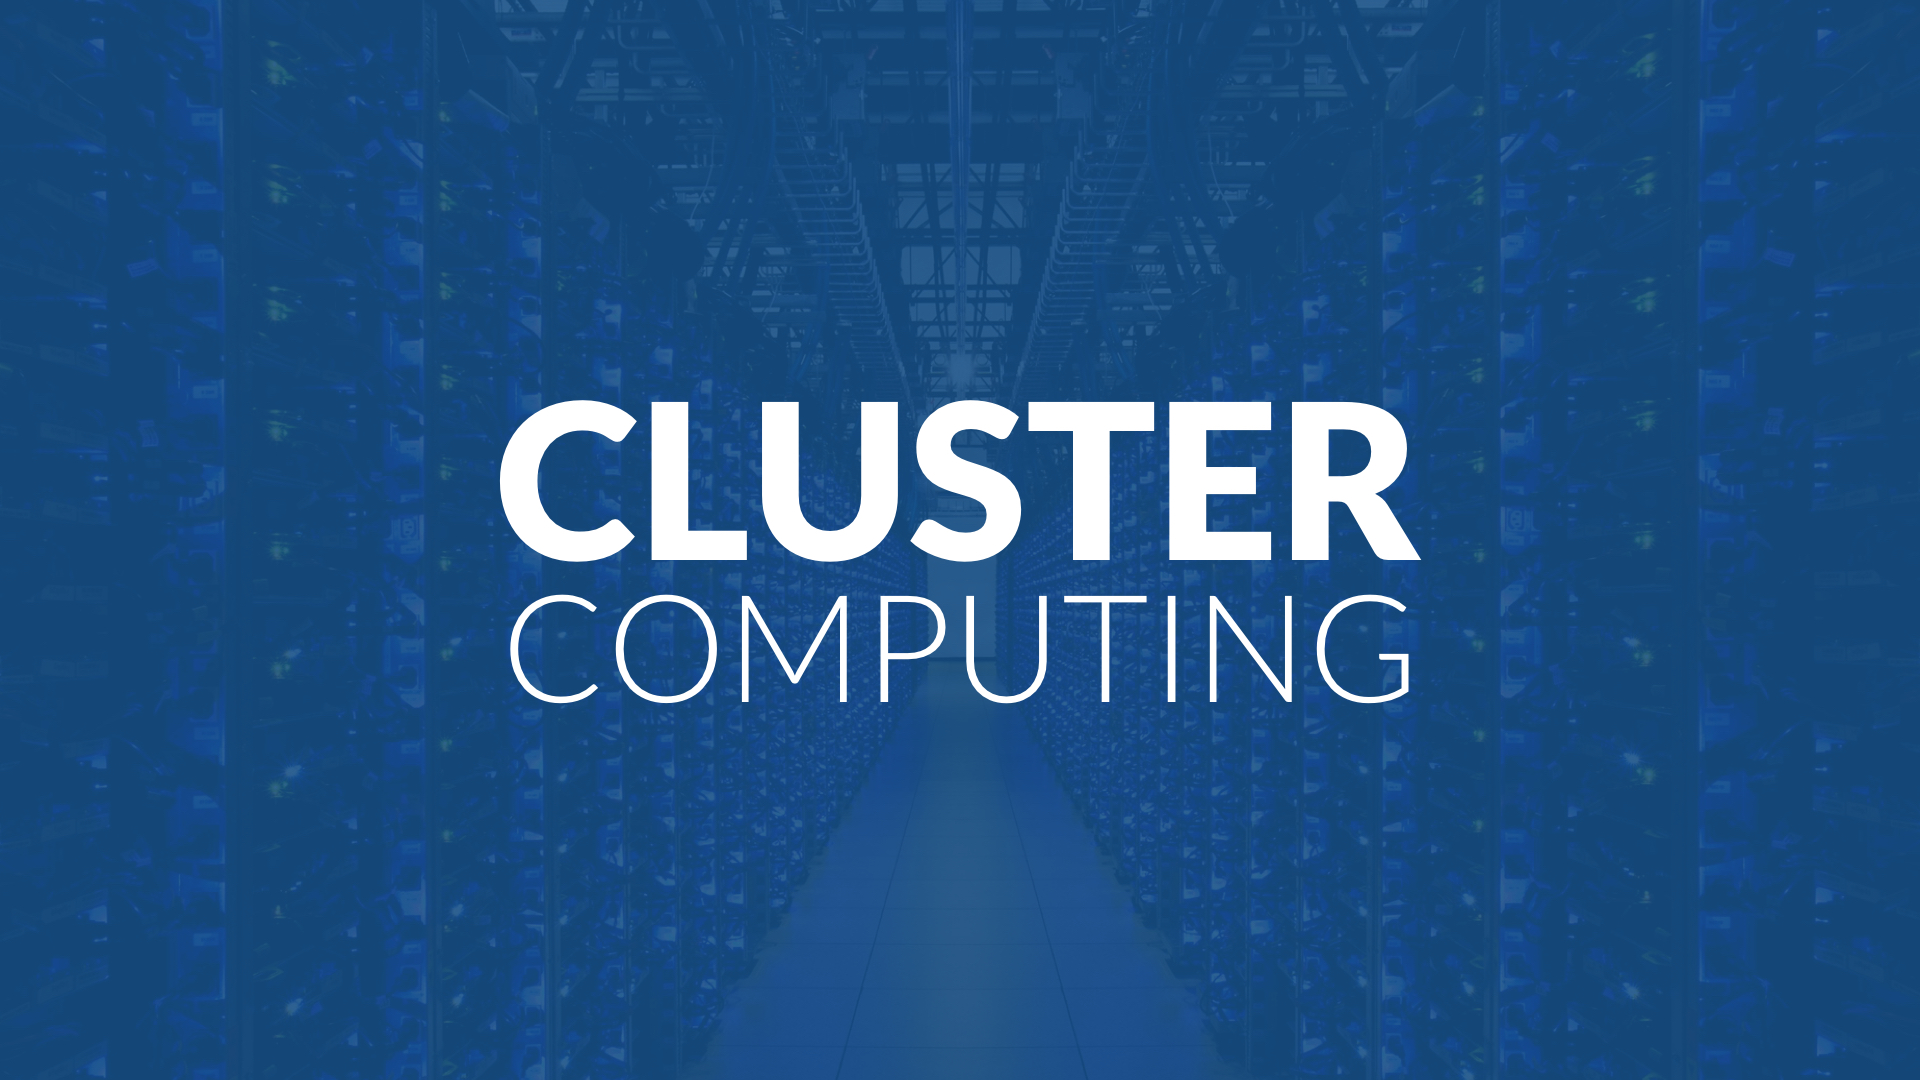
\includegraphics[align=t,width=6cm]{figures/slides/slides_w1_cluster_computing} & \textbf{Cluster Computing} \newline \textit{(18 slides)} \newline Sequential vs parallel programming. Anatomy of a Raspberry Pi cluster. Introduction to Message Passing Interface (MPI). \\ 


\includegraphics[align=t,width=6cm]{figures/slides/slide_w1_cloud_computing} & \textbf{Cloud Computing \& Microservices architecture} \newline \textit{(60 slides)} \newline Introduction to Cloud Computing, Monolithic and Microservices architecture, Continuous Delivery. \\ 
\end{tabular}
\newpage

\noindent\begin{tabular}{p{6cm}p{7.5cm}}

\includegraphics[align=t,width=6cm]{figures/slides/slides_w1_spring_cloud} & \textbf{Frameworks for microservices} \newline \textit{(21 slides)} \newline Introduction to Spring Boot and Spring Cloud. Small code examples and an overview of how to apply these tools in the project. \\ 


\includegraphics[align=t,width=6cm]{figures/slides/slides_w1_demo} & \textbf{Recap and demonstration} \newline \textit{(15 slides)} \newline Spring Boot and Spring Cloud recap and presentation of demo project to be demonstrated. \\ 
\end{tabular}

\subsection*{Module 2 - Docker Lightweight Containers}

\renewcommand*{\arraystretch}{2}
\begin{tabular}{p{6cm}p{7.5cm}}

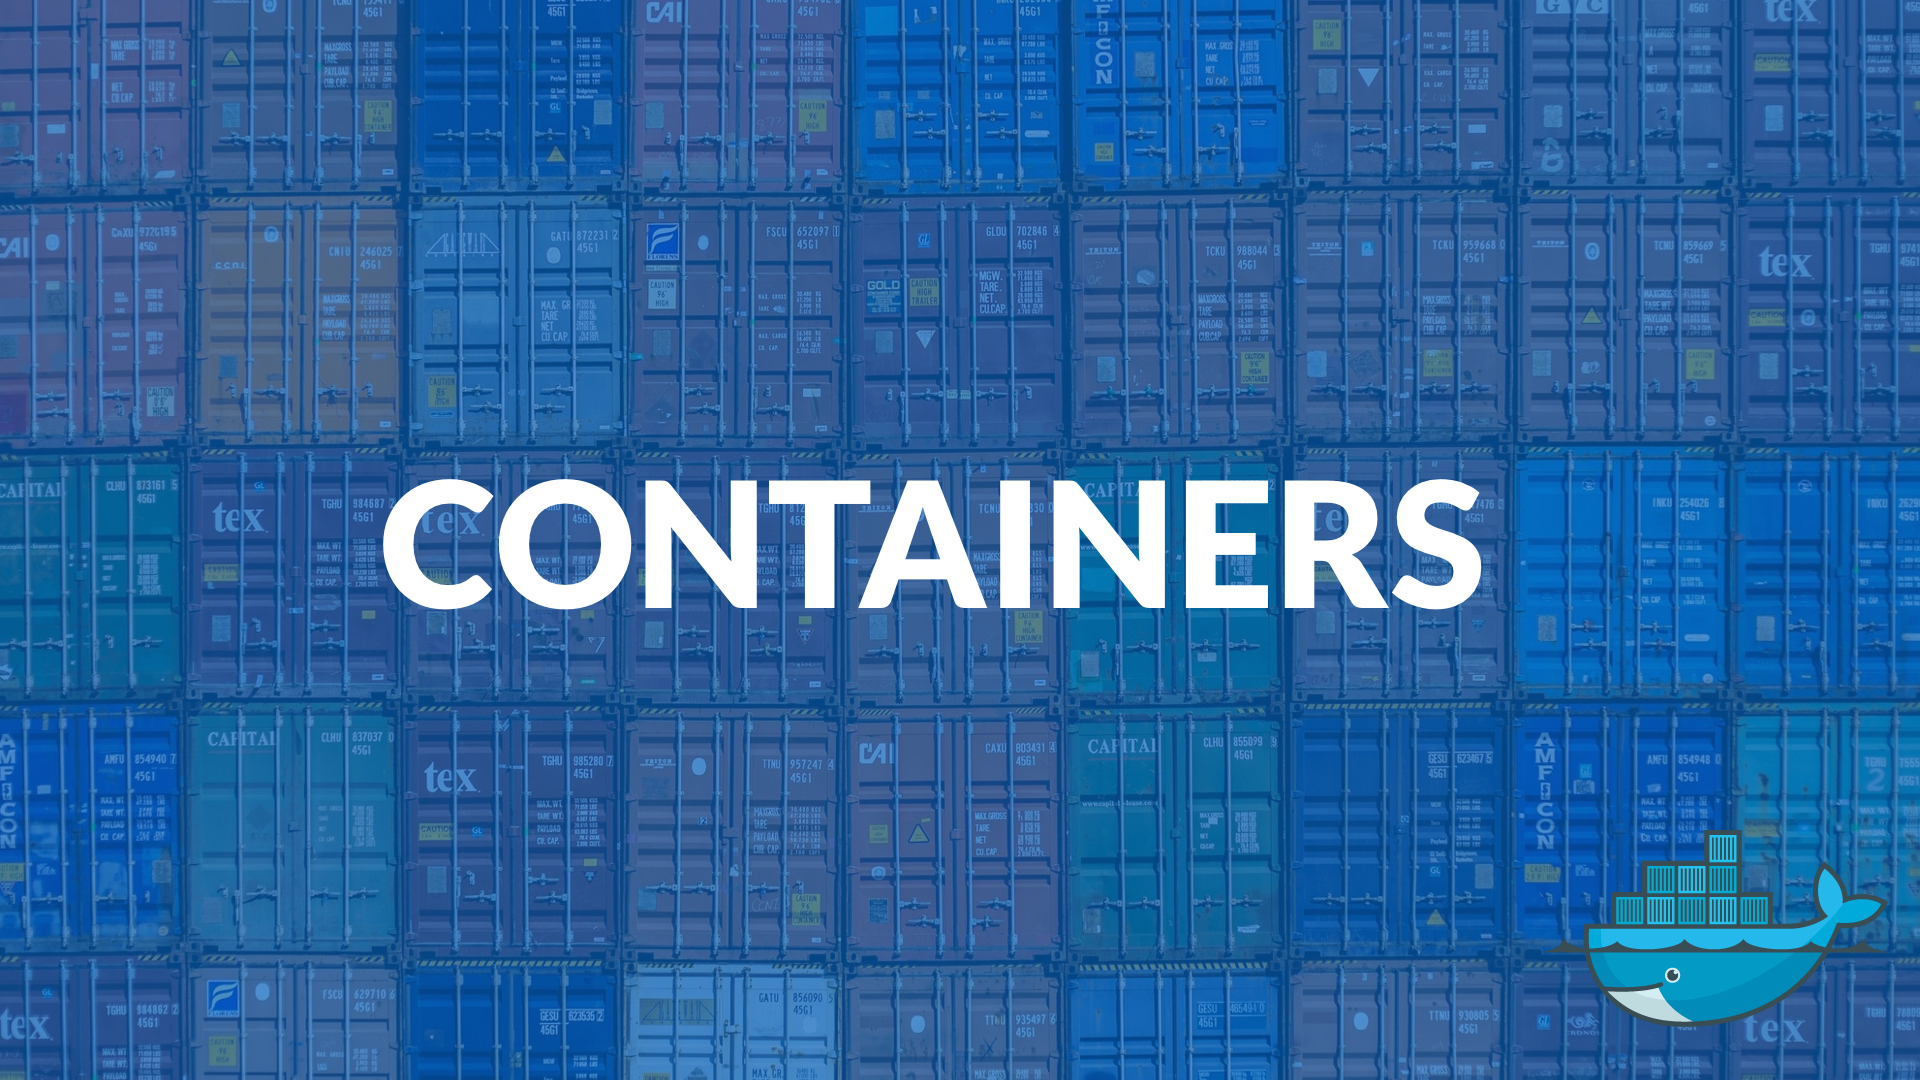
\includegraphics[align=t,width=6cm]{figures/slides/slides_w2_containers_docker} & \textbf{Containers \& Docker} \newline \textit{(21 slides)} \newline A short introduction to Docker and the challenges Docker addresses. Anatomy of a Docker container and the architecture.  \\ 

\end{tabular}


\subsection*{Module 3 - Kubernetes Cluster Manangement}
\renewcommand*{\arraystretch}{2}
\begin{tabular}{p{6cm}p{7.5cm}}

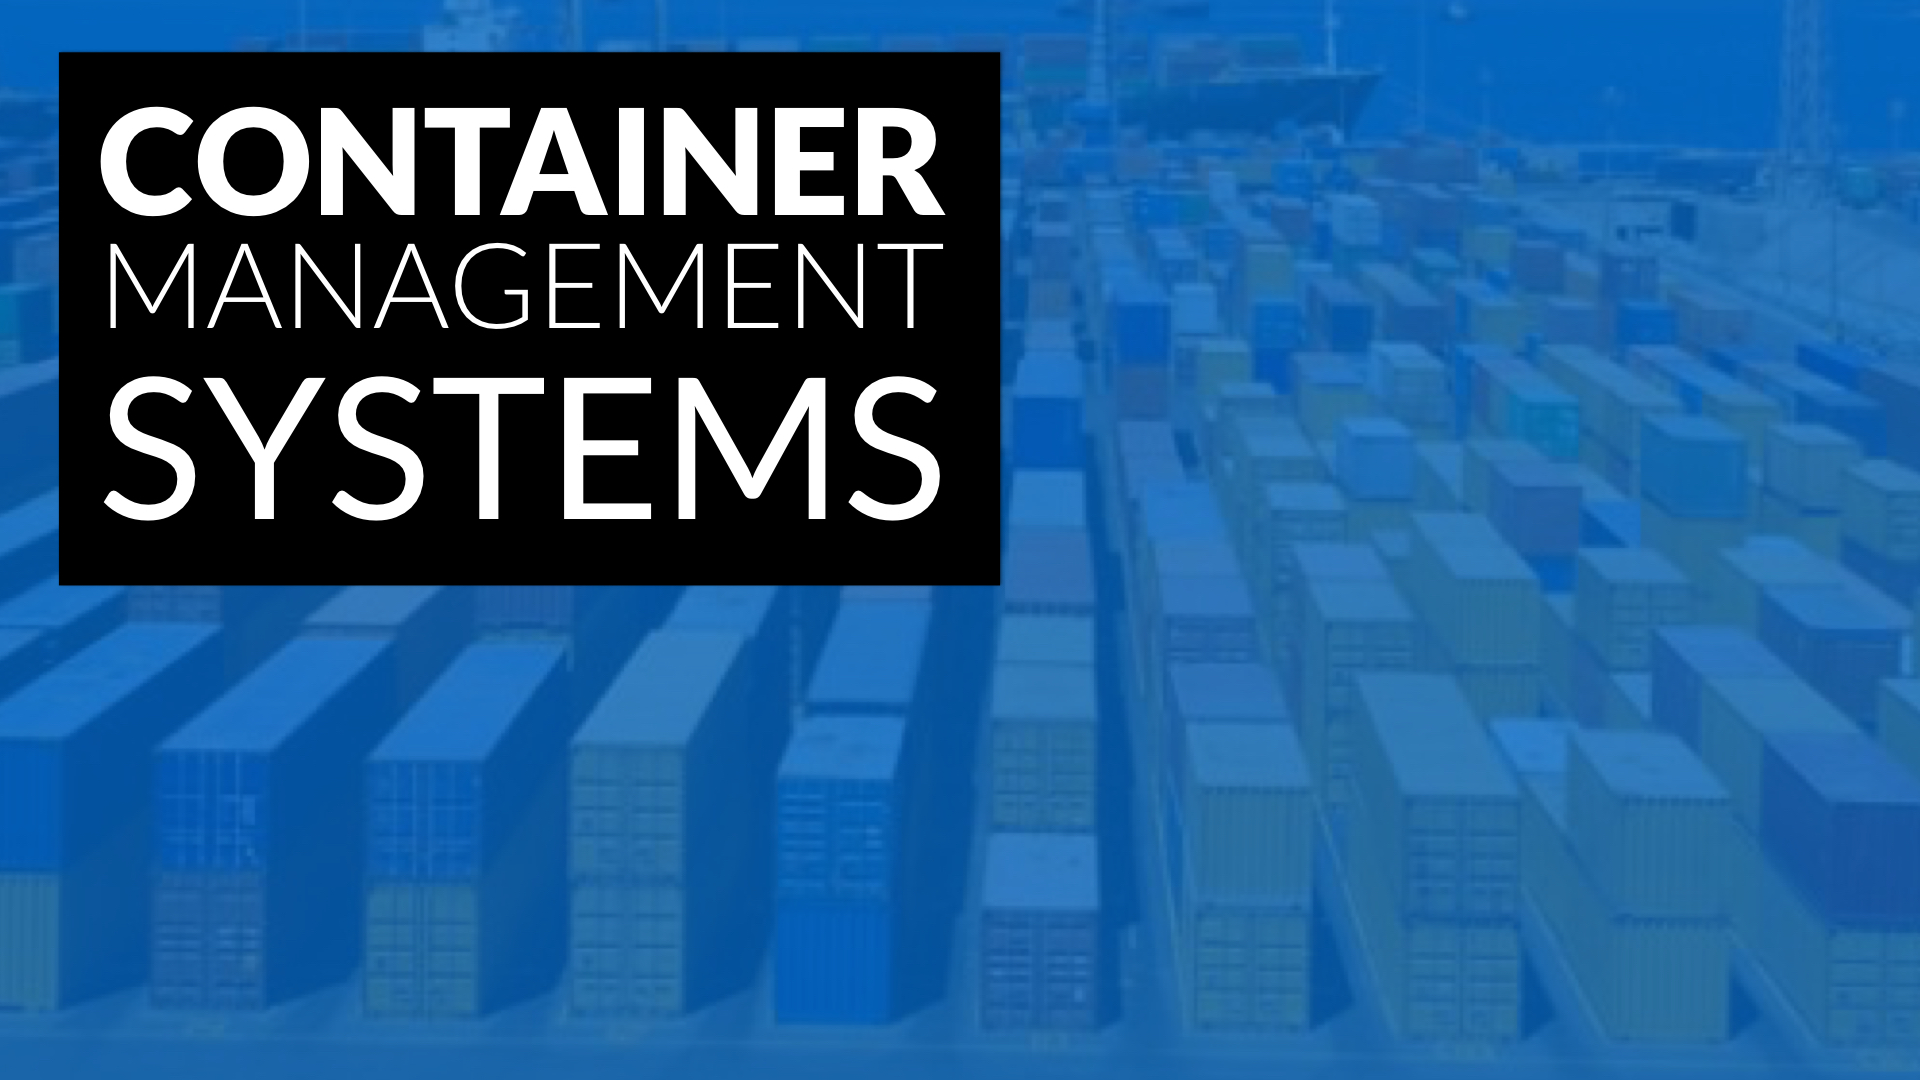
\includegraphics[align=t,width=6cm]{figures/slides/slides_w3_container_management_systems} & \textbf{Container Management systems \& Kubernetes} \newline \textit{(62 slides)} \newline Introduction to Cluster Management and a more detailed introduction to Kubernetes, its concepts and how it works from a high-level perspective. \\ 

\end{tabular}

\subsection*{Module 4 - Resilience and Load Testing}
\renewcommand*{\arraystretch}{2}
\begin{tabular}{p{6cm}p{7.5cm}}


\includegraphics[align=t,width=6cm]{figures/slides/slides_w4_resilience} & \textbf{Resilience \& Load testing} \newline \textit{(58 slides)} \newline Introduction to resilience and load testing. Focusing on Michael Nygard antipatterns and patterns.\\ 

\end{tabular}

\subsection*{Module 7 - Service Discovery}

\renewcommand*{\arraystretch}{2}
\begin{tabular}{p{6cm}p{7.5cm}}

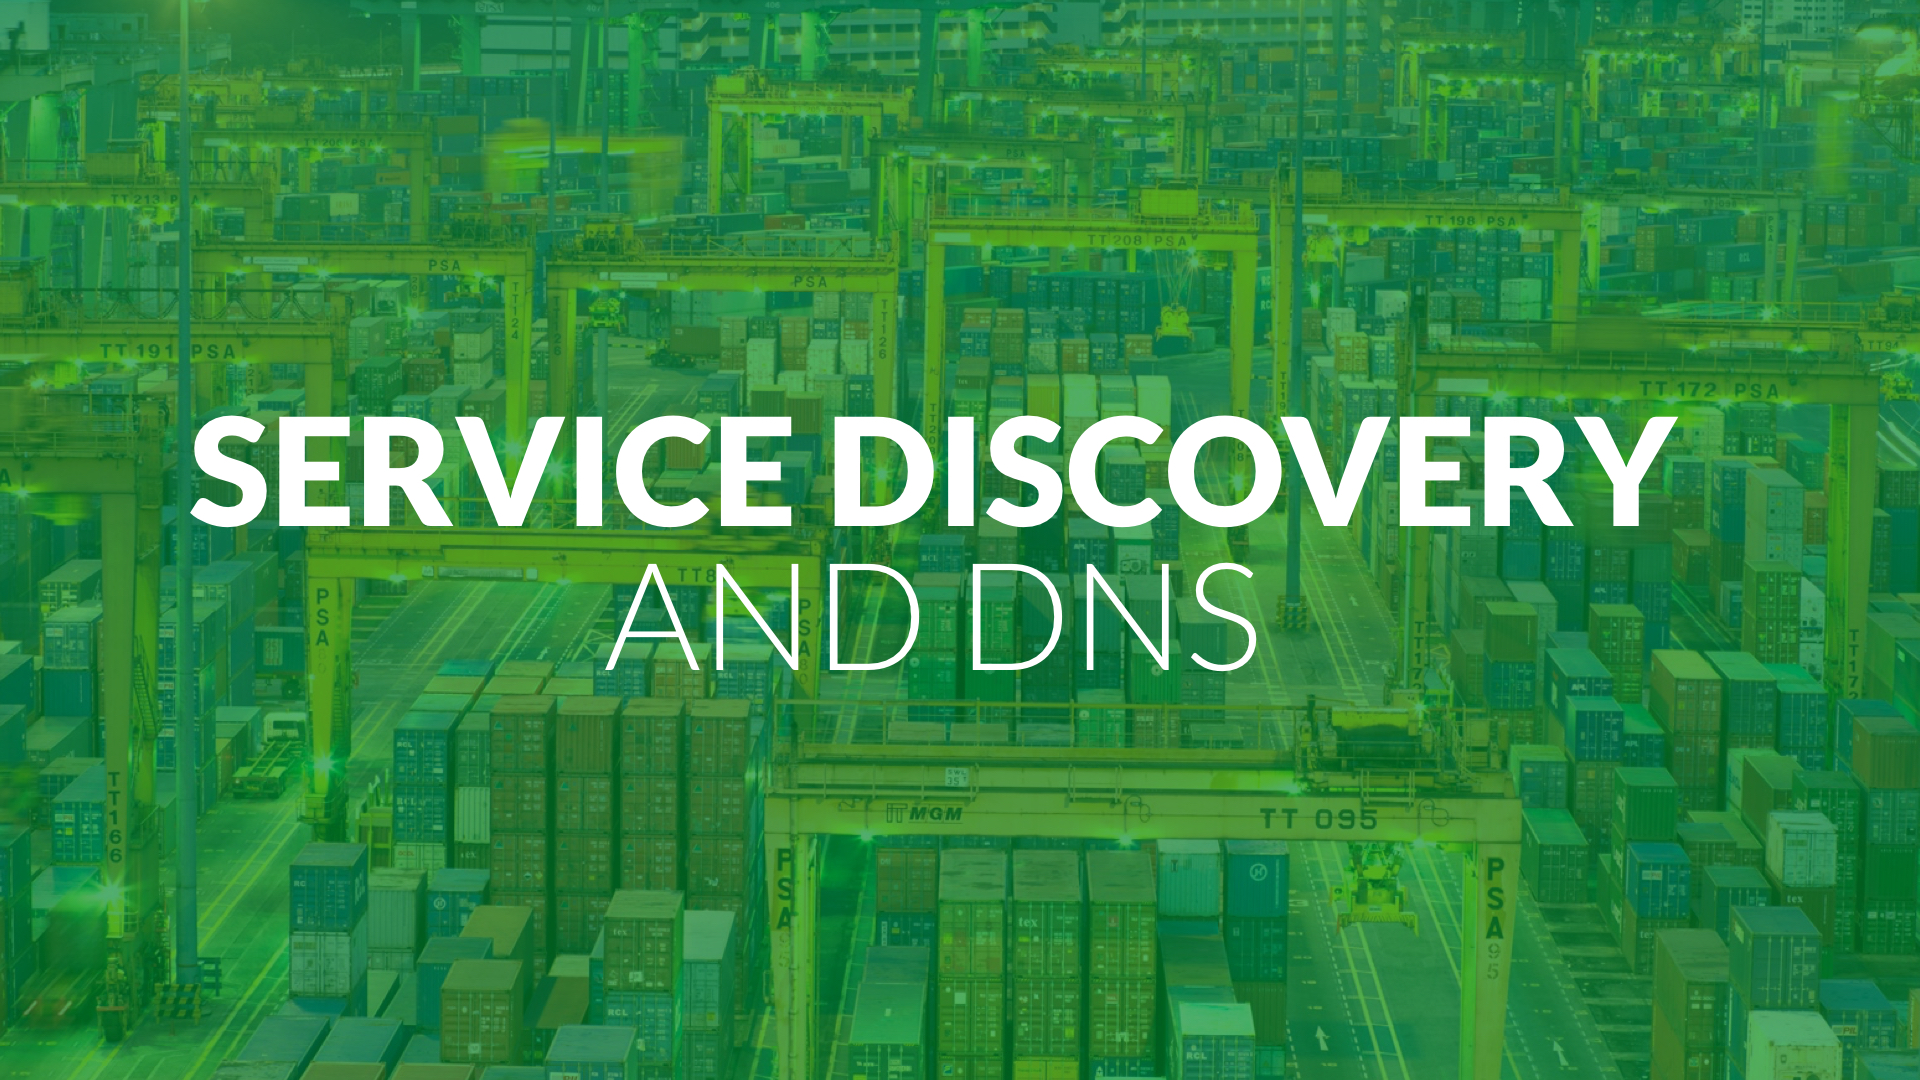
\includegraphics[align=t,width=6cm]{figures/slides/slides_w7_service_discovery} & \textbf{Service Discovery} \newline \textit{(20 slides)} \newline Introduction to client-side service discovery, server-side service discovery (Kubernetes), and course evaluation.\\ 

\end{tabular}


%\subsection*{Module 7 - Service Discovery and project presentations}